%%%%%%%%%%%%%%%%%%%%%%%%%%%%%%%%%%%%%%%%%%%%%%%%%%%%%%%%%%%%%%%%%%%%%%
% CS637: Database-Backed Websites
% Copyright 2015 Pejman Ghorbanzade <pejman@ghorbanzade.com>
% Creative Commons Attribution-ShareAlike 4.0 International License
% More info: https://github.com/ghorbanzade/beacon
%%%%%%%%%%%%%%%%%%%%%%%%%%%%%%%%%%%%%%%%%%%%%%%%%%%%%%%%%%%%%%%%%%%%%%

\section*{Question 2}

Compose a web page \texttt{register.html} with page title \textit{User Registration}, contents entitled \textit{Register for This Website}, and a form, specifying name and email addresses in a text boxes, and a having a submit button. Include the text of \texttt{register.html} and its display from a browser in your homework submission. Note that we can't make this form work yet, just see it display itself.

\subsection*{Solution}

The form has been developed on \href{http://ghorbanzade.com/cs637?p=3&s=1}{\texttt{Ghorbanzade.com/cs637}}dedicated to the course. To fully comply with what is asked by the question, a new page \href{http://ghorbanzade.com/cs637/register.html}{\texttt{register.html}} has also been developed in pure HTML and is available on the same website. Front-end of \href{http://ghorbanzade.com/cs637/register.html}{\texttt{register.html}} is depicted in Figure \ref{fig1}.

\begin{figure}[H]\centering
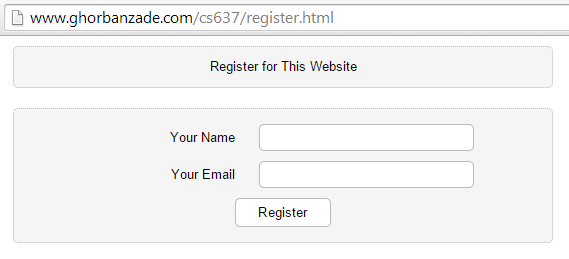
\includegraphics{\pngDirectory/hw02/hw02q02f01}
\caption{Front-End of User Registration Page}
\label{fig1}
\end{figure}

Following is the HTML code generating the web page.

\begin{lstlisting}
%\begin{minted}[fontsize=\small,tabsize=8,linenos, firstnumber=1,frame=lines,framerule=1pt]{html}
<!DOCTYPE html>
<html>
  <head>
    <meta charset='utf-8'>
    <link type="text/css" rel="stylesheet" media="all" href="temp/style/enstyle.css">
    <title>User Registration</title>
  </head>
  <body>
    <div class="pane">
      <div id='message'>Register for This Website</div>
        <form class="formNorm" method="post" action="/cs637?p=3&s=1" accept-charset="utf-8">
        <div class='field'>
          <label for="name">Your Name</label>
          <input type="text" id="name" name="name" value="" tabindex="1" required>
        </div>
        <div class='field'>
          <label for="email">Your Email</label>
          <input type="email" id="email" name="email" value="" tabindex="2" required>
        </div>
        <input type="submit" value="Register" tabindex="3">
        <input type="hidden" name="try" value="1">
      </form>
    </div>
  </body>
</html>
%\end{minted}
\end{lstlisting}

For better presentation, the following CSS style has been used.

\begin{lstlisting}
%\begin{minted}[fontsize=\small,tabsize=8,linenos, firstnumber=1,frame=lines,framerule=1pt]{css}
<style>
body {
    font-family: arial;
    font-size: 13px;
}
body .pane {
    padding: 20px 5%;
    width: 40%;
    border-radius: 10px;
    margin: 20px auto 0px;
}
body #message {
    line-height: 40px;
    text-align: center;
    border: 1px dotted #bbb;
    background-color: whitesmoke;
    border-radius: 5px;
}
body .formNorm {
    margin: 20px 0 0 0;
    background-color: whitesmoke;
    border-radius: 5px;
    border: 1px dotted #bbb;
    padding: 10px 5%;
}
body .formNorm .field {
    line-height: 30px;
}
body .formNorm .field label {
    width: 40%;
    display: inline-block;
    text-align: right;
    padding: 0 20px 0 0;
}
body .formNorm .field input:focus,
body .formNorm .field input:hover {
    outline: none;
}
body .formNorm .field input[type=text],
body .formNorm .field input[type=email] {
    display: inline-block;
    width: 40%;
    border: 1px solid #bbb;
    border-radius: 5px;
    line-height: 25px;
    padding: 0 10px;
    margin: 5px 0;
    background: white;
}
body .formNorm input[type=submit] {
    border: 1px solid #bbb;
    width: 20%;
    margin: 5px 40%;
    line-height: 25px;
    border-radius: 5px;
    background: white;
}
</style>
%\end{minted}
\end{lstlisting}

